\documentclass[a4paper]{article}
\usepackage{hyperref}
\usepackage{microtype}
\usepackage{mathpazo,xcolor}
\usepackage[top=1cm,left=1cm,right=1cm,bottom=1cm]{geometry}
\usepackage{graphicx,soul,lipsum}
\parindent0pt
\makeatletter
\def\HUGE{\@setfontsize\HUGE{65}{90}}
\makeatother
\begin{document}
\thispagestyle{empty}

% define university colors
\definecolor{cprimary}{RGB}{0,39,76}
\definecolor{csecondary}{RGB}{255,112,0}

\newcommand{\name}[1]{\textit{#1}}

\raggedbottom
\begin{minipage}{0.95\textwidth}
\sffamily
\centering
\LARGE{\color{csecondary}\bf PROBLEM SOLVING SEMINAR}\\

\Large{\color{cprimary}\textbf{\so{Department of Mathematics}}}\\

\large{\color{cprimary}\textbf{\so{California State University Fullerton}}}\\
\smallskip
\large{\color{cprimary}\textbf{{\color{csecondary}Meeting room:} MH 476}}
%\large{\color{cprimary}\textbf{\so{Zoom Meeting Room: \ref{https://fullerton.zoom.us/j/89343255295?pwd=ZFR3VThaM29ZYkdReGVQS0daS1pHUT09}{893\ 4325\ 5295}\quad Password: 112358}}}\\

\bigskip

\begin{minipage}[b]{0.47\textwidth}
\normalsize
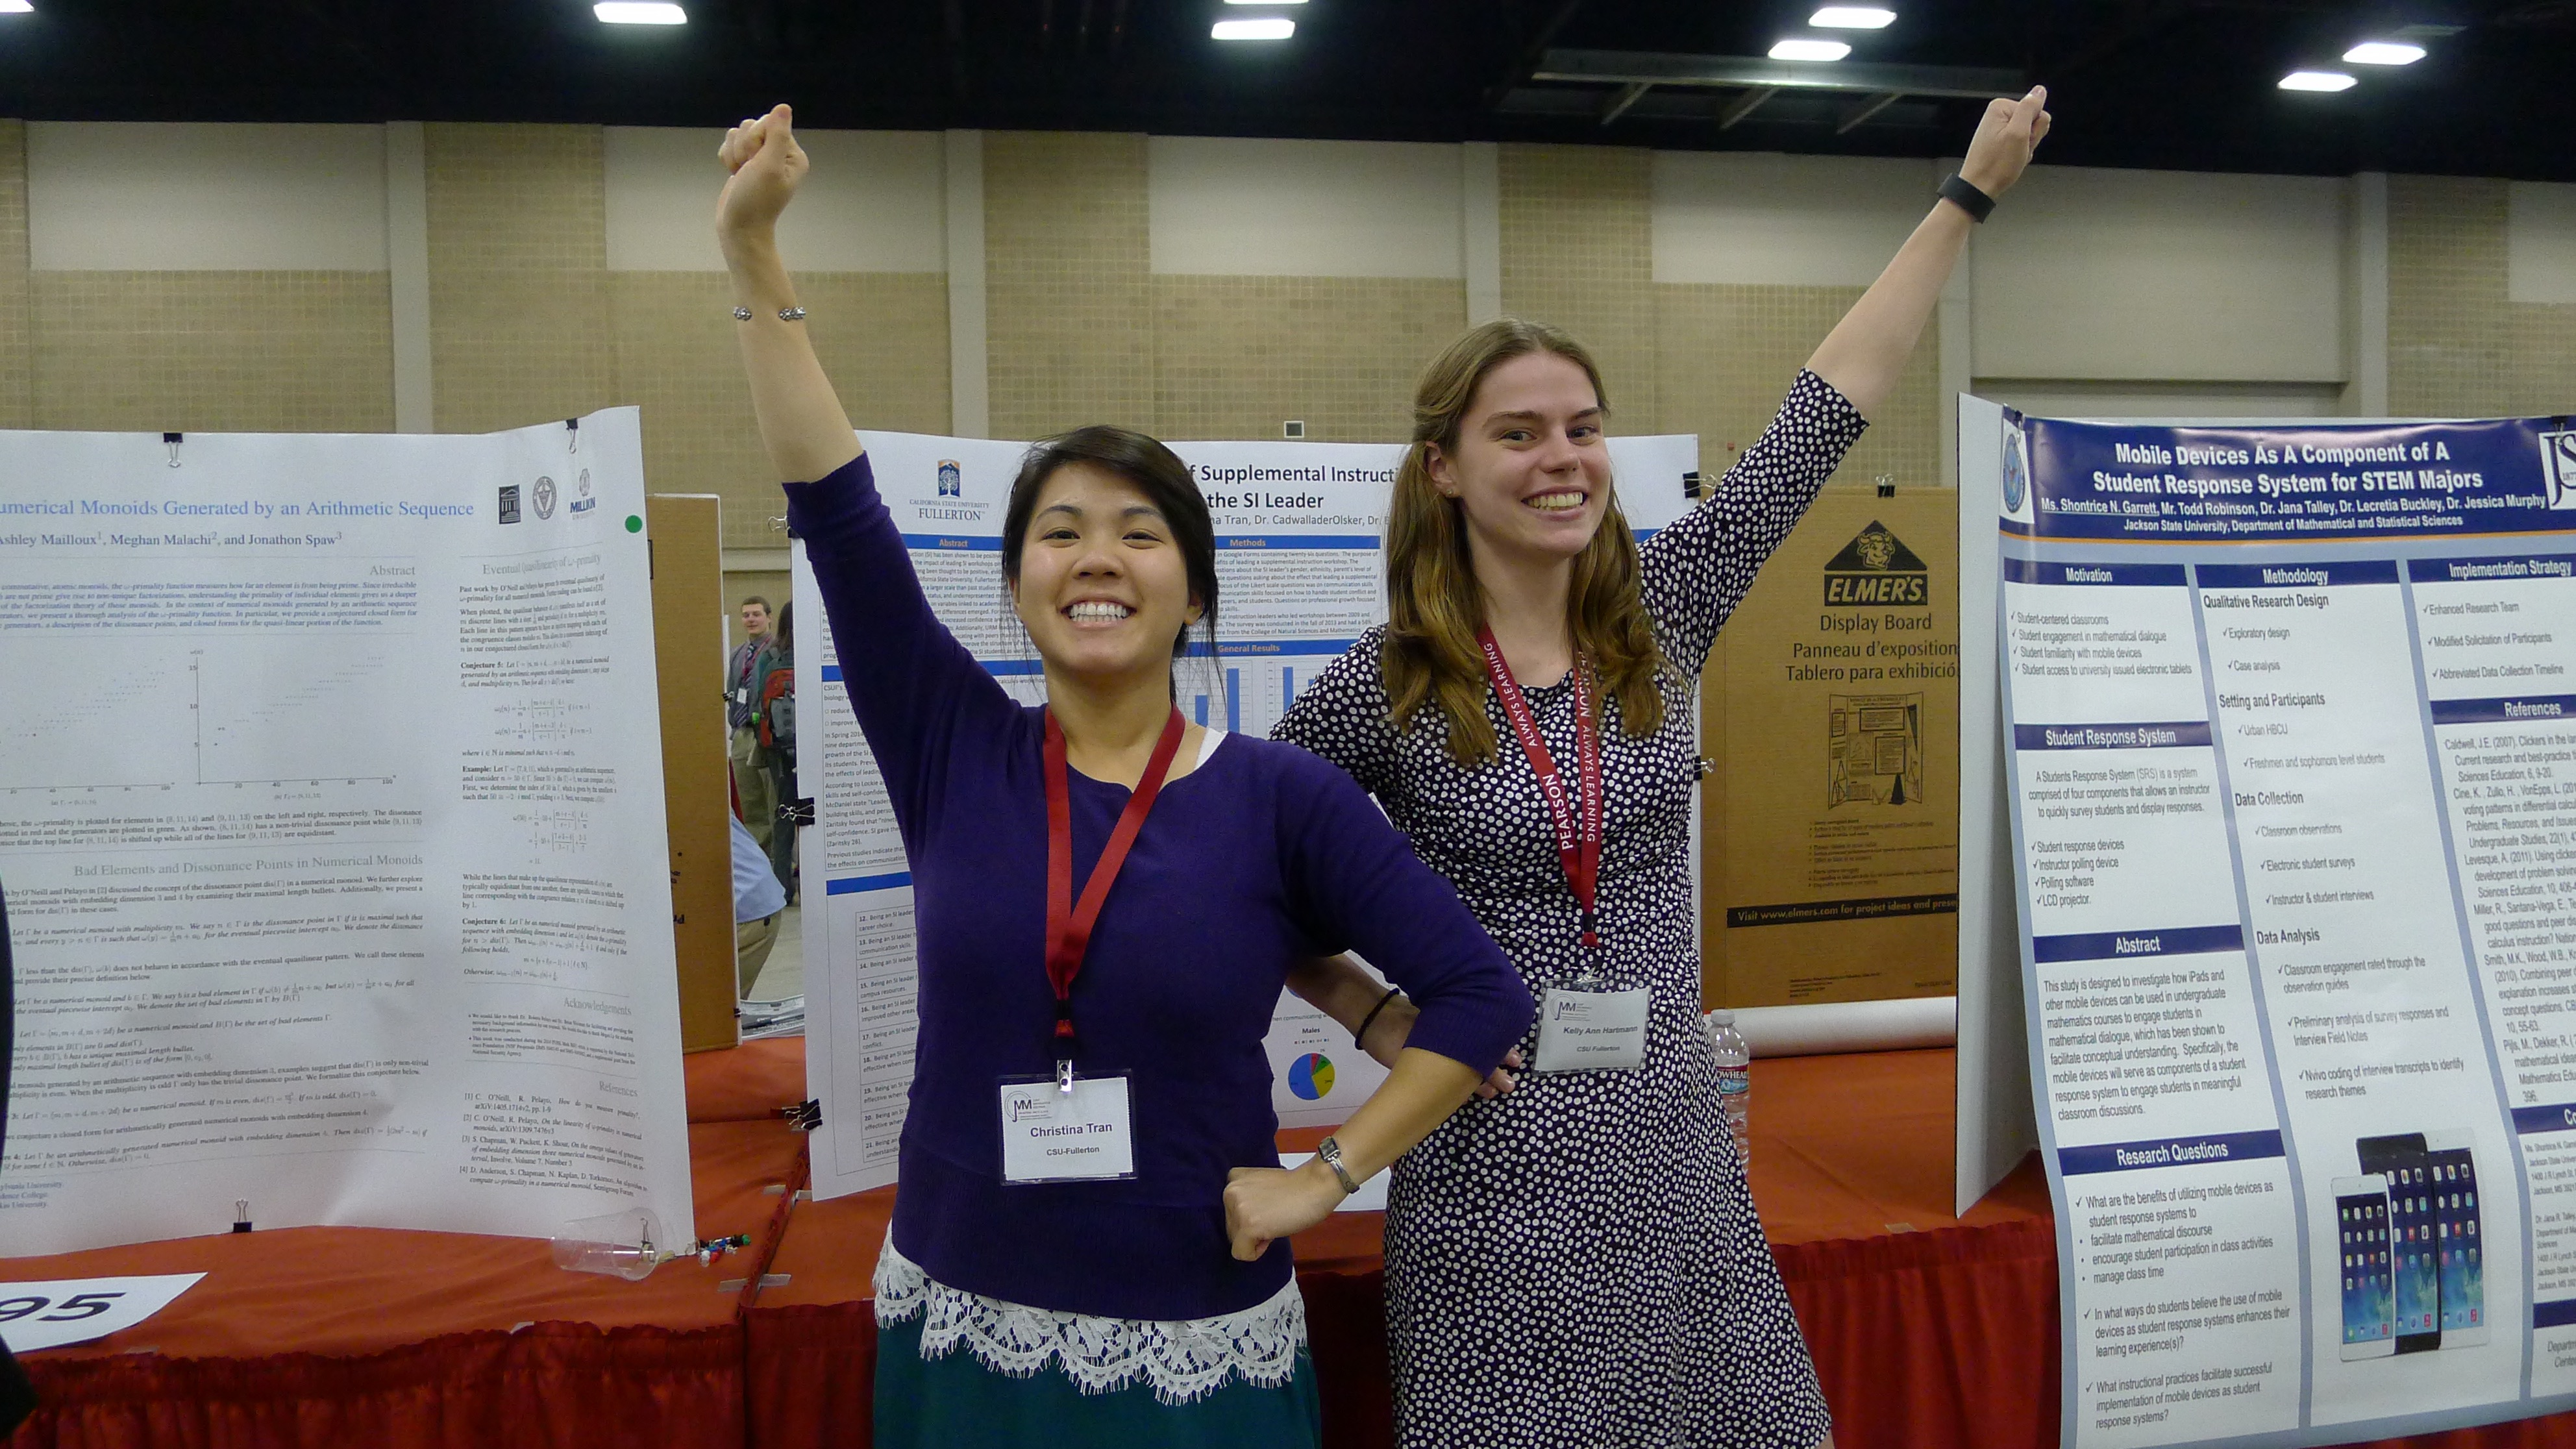
\includegraphics[width=\linewidth]{SanAntonio.jpg}
Christina Tran and Kelly Hartmann presenting the CSUF math seminars, outreach programs, and the SI program at the Joint Mathematical Meetings, San Antonio, 2015.
\medskip\par
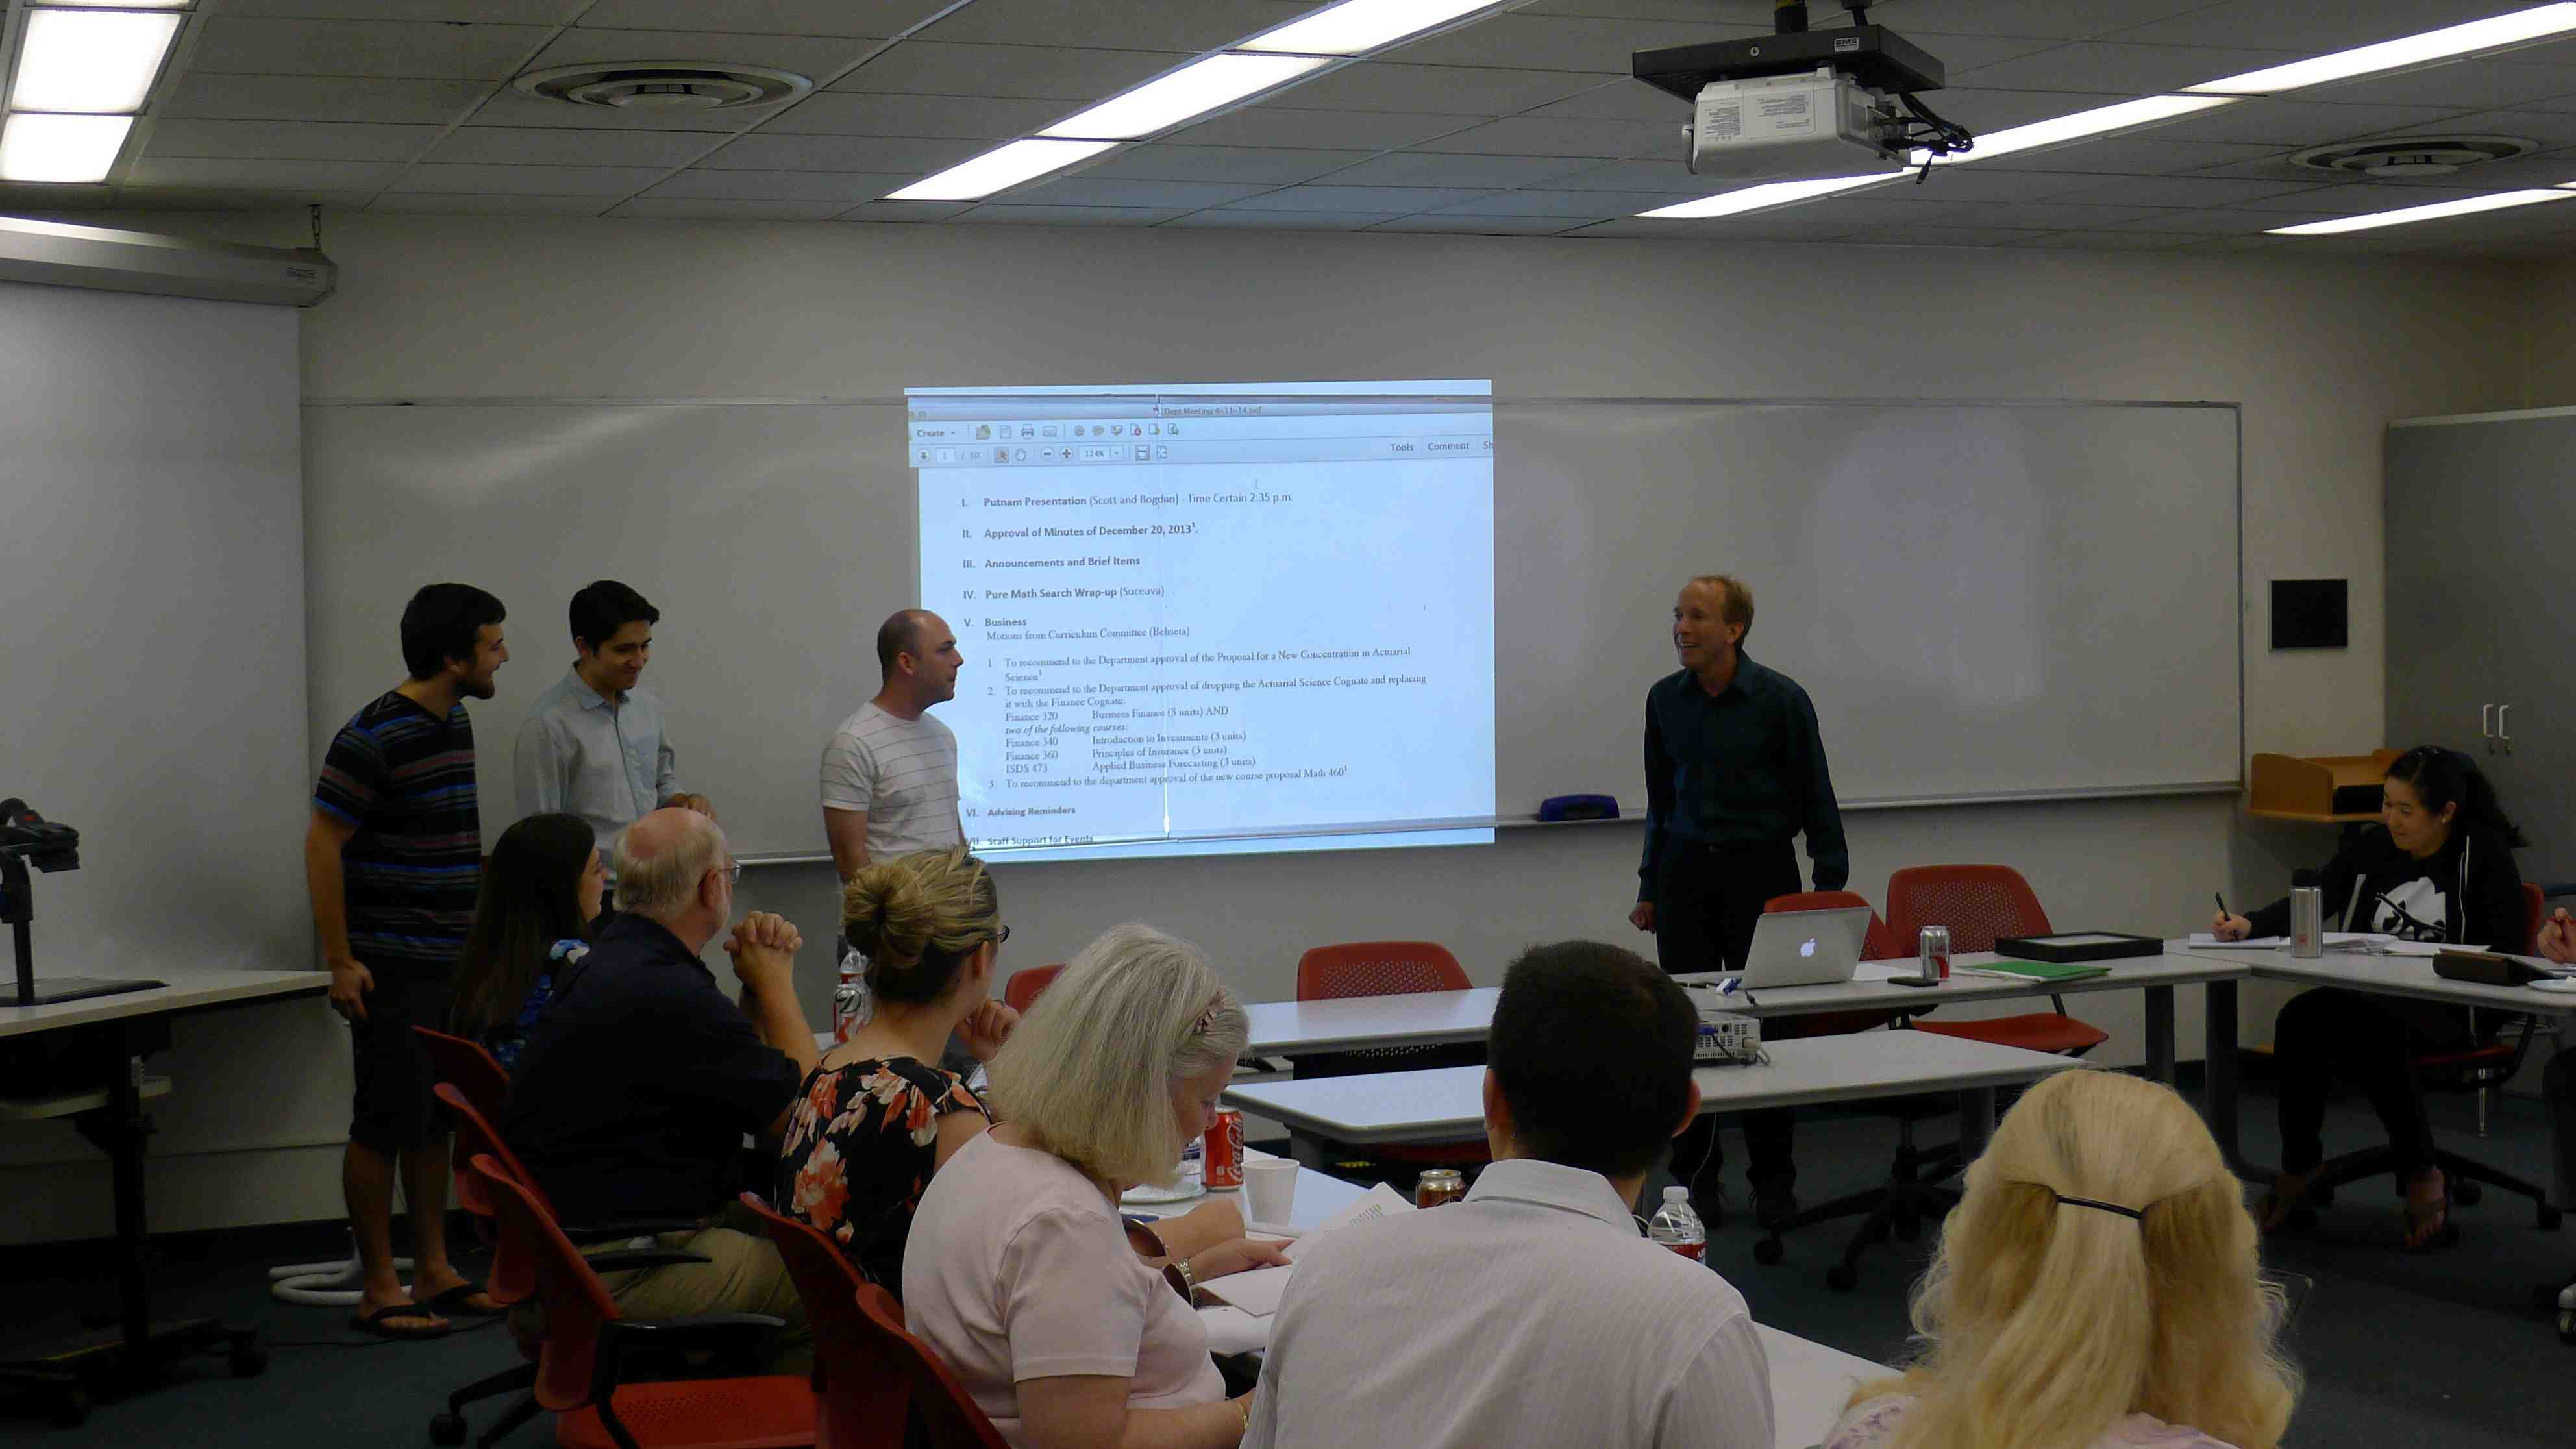
\includegraphics[width=\linewidth]{Ben.jpg}
The Department of Mathematics recognizing the outstanding performance of the 2014 CSUF Putnam team, Danny Orton, Fernando Quintino, and Ben Blazak.
\medskip
\medskip

{\large\raggedright
{\textbf{\color{csecondary}ABOUT THE SEMINAR}}\par
}
\normalsize
\smallskip

The CSUF Problem Solving Seminar traditionally engages our interested undergraduate students as they prepare for
the William Lowell Putnam Competition. Besides the content similar to these programs, we are discussing problems
from various journals, including The American Mathematical Monthly, Mathematics Magazine, the College
Mathematical Journal, Gazeta matematică, or the Mathematical Gazette (London).

\medskip

Our goal is to inform and entertain, as we enjoy exploring fundamental mathematics. Any undergraduate student is
most welcome and invited to join. All the sessions are independent from one another.

\medskip

The W.L.~Putnam Competition will take place \textbf{Saturday, December 3} from \textbf{$8$ AM to $4$ PM} in \textbf{MH 476}.
\begin{center}

\includegraphics[width=0.55\linewidth]{csuf_seal.png}
\end{center}
\smallskip

\rule{0pt}{32pt}
\end{minipage}\hspace{5pt}
\begin{minipage}[b]{0.47\textwidth}
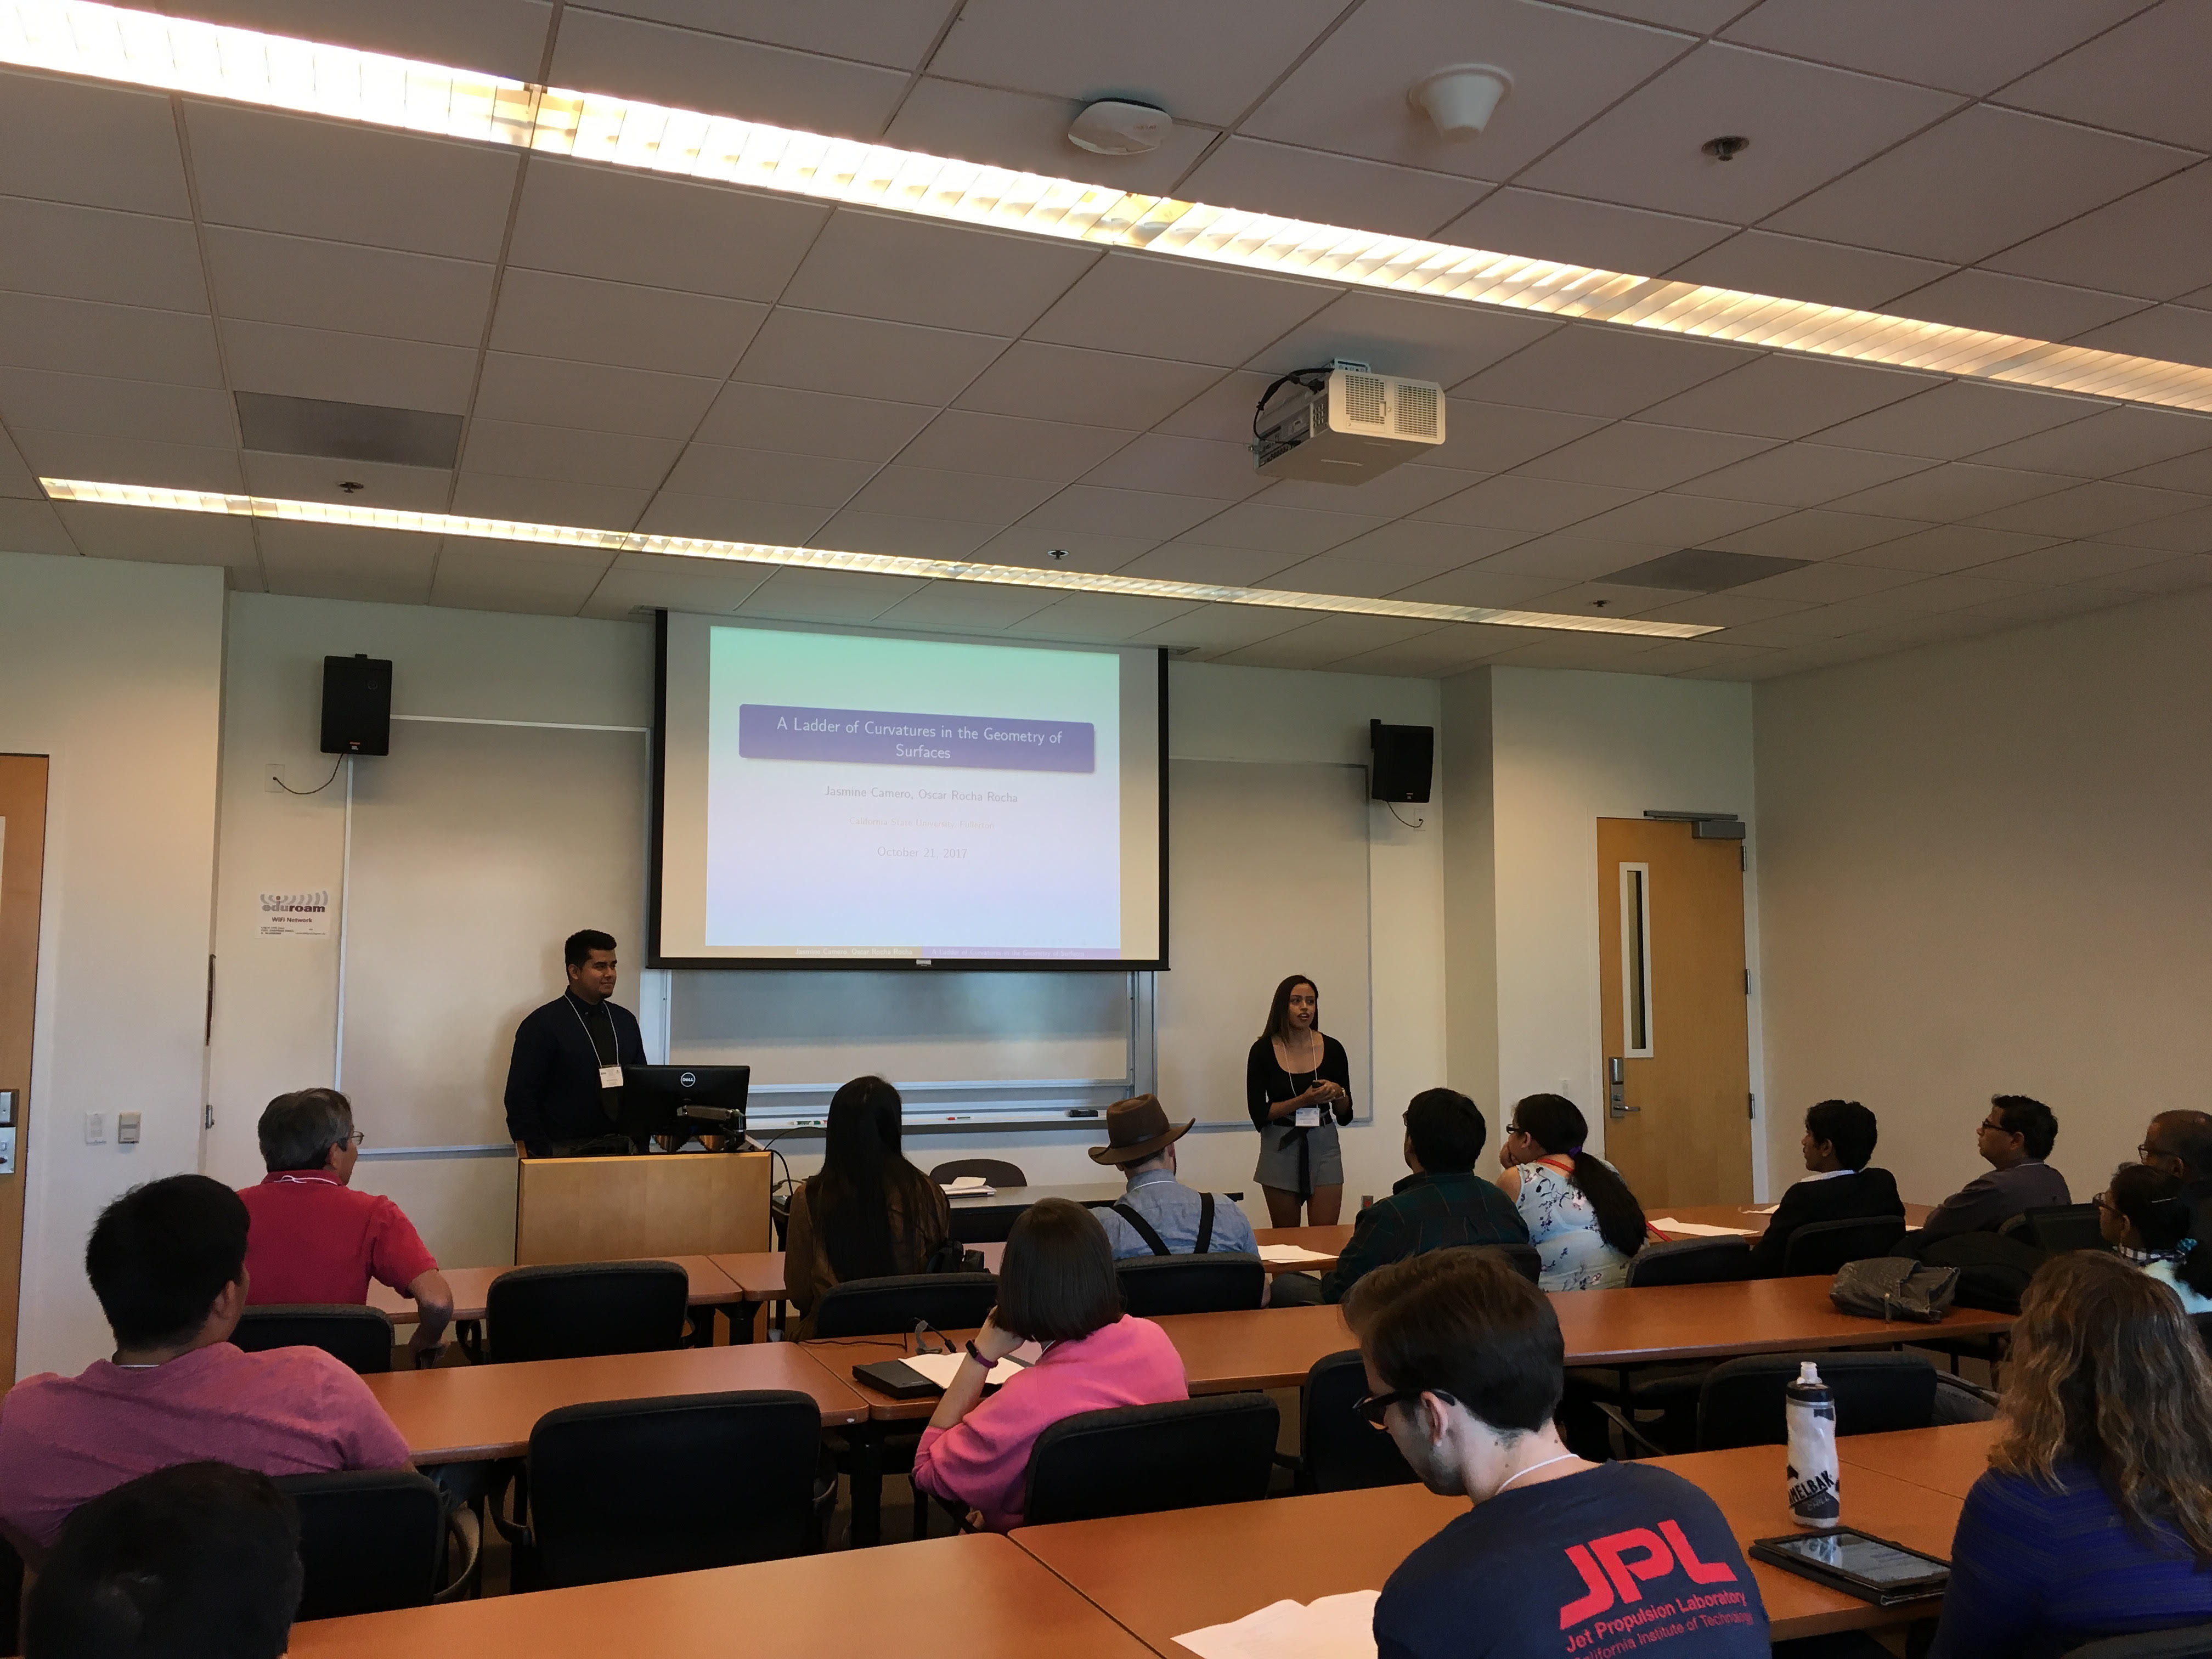
\includegraphics[width=\linewidth, trim = {0 0 0 25cm}, clip]{Oscar.jpg}
Jasmine Camero and Oscar Rocha Rocha presenting their research project at the Fall 2017 MAA Meeting, SoCal Nevada Section.
\medskip
\medskip

{\large\raggedright
{\textbf{\color{csecondary}SCHEDULED TALKS}}
}\par
\normalsize
\smallskip


{\leavevmode \raggedright
\textbf{\color{cprimary}Friday, September 2, 1:00 pm}\\ \name{Riley Casper}\\
\textbf{\color{cprimary}Friday, September 9, 1:00 pm}\\ \name{Sho Seto}\\
\textbf{\color{cprimary}Friday, September 16, 1:00 pm}\\ \name{Tommy Murphy}\\
\textbf{\color{cprimary}Friday, September 23, 1:00 pm}\\ \name{Matt Rathbun}\\
\textbf{\color{cprimary}Friday, September 30, 1:00 pm}\\ \name{Adam Glesser}\\
\textbf{\color{cprimary}Friday, October 7, 1:00 pm}\\ \name{Riley Casper}\\
\textbf{\color{cprimary}Friday, October 14, 1:00 pm}\\ \name{Sam Fleyshman and Sara Anderson}\\
\textbf{\color{cprimary}Friday, October 21, 1:00 pm}\\ \name{Kevin Nichols}\\
\textbf{\color{cprimary}Friday, October 28, 1:00 pm}\\ \name{Stephanie Reed}\\
\textbf{\color{cprimary}Friday, November 4, 1:00 pm}\\ \name{TBA}\\
%\textbf{\color{cprimary}Friday, November 11, 1:00 pm}\\ \name{TBA}\\
%\textbf{\color{cprimary}Friday, November 18, 1:00 pm}\\ \name{TBA}\\
%\textbf{\color{cprimary}Friday, November 25, 1:00 pm}\\ \name{TBA}\\
\par{}
}

\vspace{0.2in}
\medskip

\large{\color{csecondary}\textbf{VENUE}}

The symposium will take place in MH 476.

\medskip

\large{\color{csecondary}\textbf{WEBSITE}}

For more information about CSUF's Problem Solving Seminar, including recordings of past talks, visit our website at\\ \href{https://wcasper.github.io/problem-seminar/}{https://wcasper.github.io/problem-seminar/}.

\medskip
\textbf{\color{csecondary}\large 2021-2022 ORGANIZERS}\par
\name{W.~Riley Casper}, CSUF

\medskip

\textbf{\color{csecondary}\large CONTACT }\par

\name{W.~Riley Casper}, CSUF\\
Email: \href{mailto:wcasper@fullerton.edu}{wcasper@fullerton.edu}

\rule{0pt}{78pt}
\end{minipage}
\vspace*{-70pt}

\end{minipage}
\end{document}

